\chapter{Parallelization of SKPDP using Pipelining Technique}
\label{chap:pipeline}

The conventional 0/1-KPDP lends itself to a very straight-forward parallelization, because any element of a certain row of the dense table can be calculated independently of other elements of the same row, given the previous row. On the other hand, to calculate a row of the sparse table in SKPDP we use a process called \textit{Add-Merge-Kill} which is inherently sequential.

The idea of using the pipelining technique stems from the understanding that the whole row of sparse table does not have to be calculated before starting the calculation of the next row. Similar technieque is used to parallelize Unbounded KPDP \cite{Rashid2010AnEO} due to dependancy within rows. As a sparse row of the sparse table is being computed, the values can be used immediately for calculating the next row. This way each thread is responsible for calculating one row of the sparse table and each thread acts as a consumer of the values produced by the previous thread. In hardware this can be implemented as streaming input to processing elements \cite{sanjay-asap94}, but in software synchronization between threads is costly. So to minimize synchronization cost between threads the data between two consecutive threads can be shared in blocks instead of one data-point at a time. The block size is a very important parameter to be tuned in this algorithm, because too large of block size hinders parallelism and too small of a block size introduces more synchronization cost between threads.


\begin{figure}[htbp]
\centerline{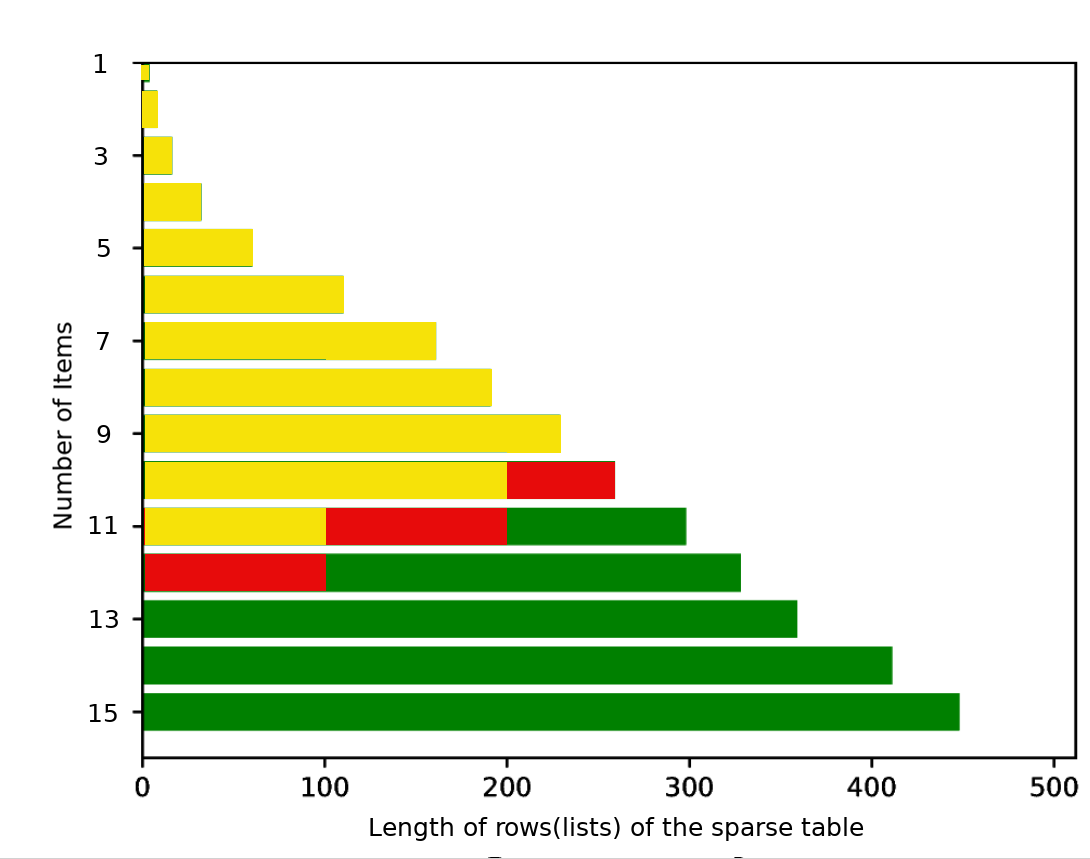
\includegraphics[width=0.8\columnwidth]{images/pipelining.png}}
\caption{Pipelining (coarse-grained) parallelism of KSPDP }
\label{fig:pipeline}
\end{figure}

Figure \ref{fig:pipeline} depicts the idea of pipelining in the context of SKPDP. Let's take a small knapsack problem instance with $N=16$ and $C=512$ for demonstration purposes. The horizontal bars represents the size of each row of the sparse table. The yellow colored parts are already calculated; the red blocks are being calculated in parallel and the green parts are yet to be calculated.

\section{Overhead Analysis} 
Most of the overhead of the computation comes from block synchronization and additional memory reads and writes of our current implementation which still requires some optimization. The worst-case space-complexity of this algorithm is $O(2NC + W_{max}P)$ because of the $P$ threads have to maintain a buffer of $w_i$. So, large values of $w_i$ hurts the performance of this technique.



\section{Implementation Details} 
Using this technique we only completely store the every $P$-th row of sparse table into memory. So, the the $(P-1)$-th thread is responsible for storing a whole sparse row, where the threads 0 to $P-2$ maintain local buffers of size $w_i$. Two very important parameters for this implementation are the block-size to be passed between threads and the thread count ($P$). Depending on the problem instance different values of block-size and thread count performs the best. We used OpenMP locks to do synchronization between the threads.


\section{Results}
We expected the course-grained technique to a do better job of parallelizing SKPDP compared to fine-grained parallelization. Figure \ref{fig:pipelined_vs_seq} shows a comparison between the complexity of corse-grained parallelization of SKPDP verses the sequential SKPDP. We observe that unlike the sequential version our implementation of the course-grained parallelization have exponential time complexity. In other words, our implementation of course-grained parallelization seem to have the same time complexity as the conventional 0/1-KPDP and we ultimately lose all the benefits of sparsity trying to parallelize the computation this way. The reason behind this behavior is yet to be discovered.

\begin{figure}[htbp]
\centerline{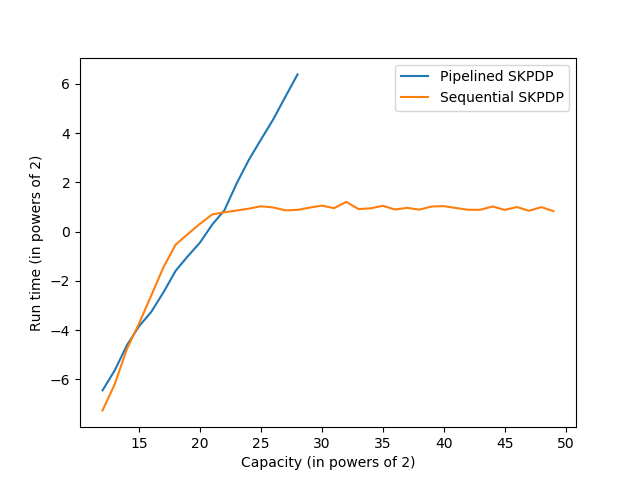
\includegraphics[width=1\columnwidth]{images/pipelined_vs_seq.png}}
\caption{Time complexity of Pipelined vs Sequential SKPDP; For all problem instances $N=256$, $noise=0.1\%$ and $W_{avg}=\frac{8C}{N}$}
\label{fig:pipelined_vs_seq}
\end{figure}